\documentclass{article}
\usepackage[utf8]{inputenc}
\usepackage[margin=1in]{geometry}
\usepackage{amsmath}
\usepackage{amsthm}
% Package for making turing machine diagrams %
\usepackage{tikz}
\usetikzlibrary{chains,fit,shapes}
% Packages for algorithms %
\usepackage{algorithm}
\usepackage{algorithmic}
% Package which has the nice looking empty set symbol (\varnothing)
\usepackage{amssymb}
% Package with the ceiling function
%\usepackage{mathtools}
%\DeclarePairedDelimiter{\ceil}{\lceil}{\rceil}
\usepackage{braket}
\usepackage{amsmath}
\usepackage{amsfonts}
\usepackage{amssymb}
\usepackage{graphicx}
\usepackage{float}

\title{Automata Theory Notes}
\author{Alex Creiner}

\theoremstyle{definition}
\newtheorem{definition}{Definition}[section]

\theoremstyle{plain}
\newtheorem{example}{Example}[section]

\theoremstyle{theorem}
\newtheorem{fact}{Fact}[section]
\newtheorem{lemma}{Lemma}[section]
\newtheorem{theorem}{Theorem}[section]
\newtheorem{corollary}{Corollary}[section]
\newtheorem{claim}{Claim}[section]


\begin{document}


\maketitle
\section{Strings and Languages}
An \textbf{alphabet} $\Sigma$ is a finite collection of symbols. Examples include the \textbf{Roman alphabet} $\{a,b,c,...,z\}$ and the \textbf{binary alphabet} $\{0,1\}$. A \textbf{string} over an alphabet is a finite sequence of symbols from the alphabet. I.e. $watermelon$ is a string over the Roman alphabet, and $01001111$ is a string over the binary alphabet. We let $|w|$ denote the \textbf{length} of the string, i.e. the number of characters. Technically, strings are functions $w: \{1,2,...,|w|\} \to \Sigma$, where if $w(i) = \sigma$, then the $i^{th}$ symbol of $w$ is the character $\sigma$. We allow strings to have no symbols at all, and denote the empty string with the letter $\epsilon$. Also, single characters can also be viewed as strings, i.e. $\sigma \in \Sigma$ can be viewed as either a character or a length $1$ string. We will let $\Sigma^*$ denote the set of all strings over the alphabet $\Sigma$. Two strings over the same alphabet can be combined via an operation called \textbf{concatenation}. If $x,y$ are strings, then the concatenation of $x$ and $y$ is denoted either $x;y$ or $x^y$ or $x \circ y$ or simply $xy$, is simply the string $x$ followed by the string $y$. More formally, $xy$ is the function $w:\{1,2,...,|x|+|y|\} \to \Sigma$ such that for $j=1,...,|x|$ $w(j)=x(j)$, and for $j=|x|+1,...,|x|+|y|$, $w(j) = y(j-|x|)$. The following fact spell out the elementary properties of string concatenation as a binary operation.
\begin{fact}
	The empty string $\epsilon$ is the identity, i.e. $x;\epsilon = \epsilon;x = x$. Furthermore, string concatenation is associative. That is, $(xy)z = z(xy)$ for all strings $x,y,z$ over an alphabet $\Sigma$. String concatenation is not, however, commutative. 
\end{fact}
\begin{proof}
	That $\epsilon$ is the identity is trivial, as is that it is not commutative. As a counterexample to commutativity, consider the string $creiner$ over the Roman alphabet. We can view this string as the concatenation of, say, $x = crei$, and $y=ner$, in which case $creiner = x;y$ but $y;x = nercrei \neq creiner$. For associativity, consider $(xy)z$ and $x(yz)$ as a functions. Both are clearly strings of length $|x|+|y|+|z|$. For $j < |x|$, $(xy)z(j) = x(j) = x(yz)(j)$. Clearly the situation is identical if $|x| < j < |x|+|y|+|z|$, so clearly these strings are the same. 
\end{proof}
We say a string $v$ is a \textbf{substring} of a string $w$ if there exist strings $x,y$ such that $v = xvy$. Note that both $x$ and $y$ could be the empty string $\epsilon$, so every string is a substring of itself. Furthermore, since for any string $w$, $w = w;\epsilon;\epsilon$, we see that the empty string is a substring of every string. Two special types of substrings are \textbf{suffixes} and \textbf{prefixes}. $v$ is a prefix of $w$ if $w = vx$ for some $x$, and is a suffix of $w$ if $w = xv$ for some $v$. 
\par Let $n \in \mathbb{N}$. We define what are essentially powers of the string $x$, $x^n$ via $x^0=\epsilon$, and $x^{n+1} = x^n;x$. Thus $x^5 = x;x;x;x;x$, and so forth. We can also define the \textbf{reversal} of a string, $x^R$, to be the string $x$, but backwards. Formally, we define the reversal of a string inductively on it's length: for strings of length $0$, i.e. $\epsilon$, $\epsilon^R = \epsilon$. If $x$ is a string of length $n+1$, then $x = y;a$ for some $a \in \Sigma$, and we define $x^R = (y;a)^R = a;y^R$. A somewhat interesting property of the reversal operation is the following:
\begin{fact}
	Let $x,y$ be strings. We have the following facts about the reversal and power operations:
	\begin{itemize}
	\item[(a)] $x,y$, $(xy)^R = y^Rx^R$.
	\item[(b)] $x$, $(x^R)^R = x$.
	\item[(c)] For any $n \in \mathbb{N}$, $(x^n)^R = (x^R)^n$
	\item[(d)] If $v$ is a substring of $w$, then $v^R$ is a substring of $w^R$
	\end{itemize}
	 Also, 
\end{fact}
\begin{proof}
	To prove (a), we induct on the length of the second string $y$. If $|y|=0$, i.e. $y=\epsilon$, then $(xy)^R =(x;\epsilon)^R = x^R = \epsilon;x^R = \epsilon^R;x^R = y^Rx^R$. Now for the inductive step, suppose that $(xy)^R = y^Rx^R$ for any strings $x$ and any strings $y$ of length less than or equal to $n$  for some $n$. Then for $y = z;a$, where $|z| = n$, we have 
	\begin{align}
		(xy)^R &= (x(za))^R = ((xz)a)^R = a(xz)^R \\
			&= a(z^Rx^R) = (za)^Rx^R = y^Rx^R
	\end{align}
Thus we have (a) by induction. For (b), again we induct on the length of $x$. If $x = \epsilon$, then of course we have $(\epsilon^R)^R = \epsilon^R = \epsilon$. Now assume that the statement holds for strings of length $n$. Then for a string $x$ of length $n$ with one extra character appended, $a$, we have
\begin{align}
	((xa)^R)^R = (ax^R)^R = (x^R)^Ra^R = xa
\end{align}
where the transitions from step two to step three follows from property (a), and step three to step four follows from the inductive hypothesis. Thus we have (b). For (c), we induct on $n$. For $n=0$, $(x^0)^R = \epsilon^R = (\epsilon^R)^0 = (x^R)^0$. Now assuming the statement holds for strings of length $n$, we have
 \[ (x^{n+1})^R = (x^n;x)^R = x^R(x^n)^R = x^R(x^R)^n = (x^R)^{n+1} \]
 Thus we have (c) by induction. Finally for (d), if $v$ is a substring of $w$, then $w = xvy$ for some strings $x,y$, and so  \[ w^R = (xvy)^R = ((x(vy))^R = (vy)^Rx^R = y^Rv^Rx^R \] From this we can clearly see that $v^R$ is a substring of $w^R$. 
\end{proof}

\begin{definition}
	A \textbf{language} is any subset $L \subseteq \Sigma^*$. 
\end{definition}
Note that since alphabets are finite, the set of all strings over an alphabet is countably infinite, and we will assume that the reader is familiar with the standard way in which to lexicographically enumerate all of these. Just as we can concatenate strings, we can also concatenate languages: If $L_1$ and $L_2$ are languages, we define
\[ L_1;L_2 = L_1 \circ L_2 := \{w \in \Sigma^*: w = x;y \textrm{ for some }x \in L_1, y \in L_2\} \]
So the concatenation of two languages is just the collection of all concatenations of strings in $L_1$ with strings in $L_2$. Note that just as the concatenation of strings is absolutely not commutative, neither is the concatenation of language; order certainly matters. We state the algebraic properties of language concatenation below. 
\begin{fact}
	Fix an alphabet $\Sigma$. We have the following:
	\begin{itemize}
		\item[(a)] String concatenation is associative. I.e. for all languages $L_1,L_2,L_3$, $L_1 \circ (L_2 \circ L_3) = (L_1 \circ L_2) \circ L_3$.
		\item[(b)] Let $\emptyset$ denote the empty language (which is not the same thing as the empty string $\epsilon$!) Then for any language $L$, $\emptyset \circ L = L \circ \emptyset = \emptyset$. Furthermore, we have that $\{\epsilon\} \circ L = L \circ \{\epsilon\} = L$. 
		\item[(c)] Concatenation of languages distributes over unions. That is, if $L_1,L_2,L_3$ are languages, then $L_1 \circ (L_2 \cup L_3) = (L_1 \circ L_2) \cup (L_1 \circ L_3)$, and $(L_1 \cup L_2) \circ L_3 = (L_1 \circ L_3) \cup (L_2 \circ L_3)$. 
	\end{itemize}
	With these results it follows that the collection of languages over $\Sigma$ forms a semiring with addition defined to be the union operation, with additive identity $\emptyset$, and multiplication defined to be concatenation with multiplicative identity $\{\epsilon\}$. 
\end{fact}
\begin{proof}
	For (a), note simply that 
		\begin{align}
		 L_1 \circ (L_2 \circ L_3) &= \{x;w: x \in L_1 \wedge w \in L_2 \circ L_3 \} \\
		 		&= \{ x;(y;z): x \in L_1 \wedge y \in L_2 \wedge z \in L_3 \} \\
		 		&= \{ (x;y);z: x \in L_1 \wedge y \in L_2 \wedge z \in L_3 \} \\
		 		&= \{ w;z: w \in (L_1 \circ L_2) \wedge z \in L_3 \} \\
		 		&= (L_1 \circ L_2) \circ L_3
		\end{align}
	Claim (b) should be fairly clear. For (c), we will prove the left distributive property, since the other is identical. Again, this is clear from direct computation:
	\begin{align}
		L_1 \circ (L_2 \cup L_3) &= \{x;y: x \in L_1 \wedge (y \in L_2 \vee y \in L_3)\} \\
		&= \{x;y: (x \in L_1 \wedge y \in L_2) \vee (x \in L_1 \wedge y \in L_3) \} \\
		&= \{x;y: x \in L_1 \wedge y \in L_2\} \cup \{x;y: x \in L_1 \wedge y \in L_3\} \\
		&= (L_1 \circ L_2) \cup (L_1 \circ L_3)	
	\end{align}
\end{proof}
We can also define the \textbf{Kleene star} of a language $L$, something we have already partially done. Note that for an alphabet $\Sigma$, we can also interpret the alphabet itself as a language - it's simply the language of single character strings. From this, we defined $\Sigma^*$ to be, effectively, the set of strings which are created from concatenating finitely many strings from $\Sigma$. We can extend this definition to languages:
 \[ L^* = \{w \in \Sigma^*: w = x_1;x_2;\ldots ;x_k \textrm{ for some }x_1,...,x_k \in L\} \]
I.e. the Kleene star of a language $L$ over an alphabet $\Sigma$ is itself a language over $\Sigma$ - it's the language created by viewing $L$ itself as an alphabet, and creating strings out of that new alphabet. Note that the Kleene star of the empty language is nonempty! $\emptyset^* = \{\epsilon\}$. However, the Kleene star of this set is itself - concatenating $\epsilon$ with itself any number of times just results in $\epsilon$ again, and so $\{\epsilon\}^* = \{\epsilon\}$. We next state some trivially true but noteworthy facts about the Kleene star operator:
\begin{fact}
	Let $\Sigma$ be an alphabet. Then we have the following:
	\begin{itemize}
		\item[(a)] $\{\epsilon\}^* = \{\epsilon\}$
		\item[(b)] If $L_1, L_2$ are languages with $L_1 \subseteq L_2$, then $L_1^* \subseteq L_2^*$. 
		\item[(c)] The empty \textit{language} $\emptyset$ is the identity for language concatenation. I.e. for any language $L$, $\emptyset;L = L;\emptyset = L$. 
	\end{itemize}
\end{fact}
The proofs of these are all trivial. Next, note that no matter what, $L^*$ includes the empty string $\epsilon$. This distinguishes $L^*$ from the operation we will denote $L^+$, and define by $L^+ := L;L^*$. Note that $L^* = L^+ \cup \{\epsilon\}$.
Now, for any set $A$, a \textbf{binary relation} is just a subset $R$ of the product $A \times A$. If there are few enough pairs in the relation $R$ (namely, finitely many) then we can always choose to view the relation $R$ as a directed graph: simply draw and label a point for each element $A$ which belongs to a pair in $R$, and then if $(a,b) \in R$, we draw an arrow from point $a$ to point $b$. Thus, at least in principle, every function and binary relation on any set, whether it be functions $f:\mathbb{R} \to \mathbb{R}$ or whatever, can be viewed as directed graphs in this way. Thus, we can very generally define the \textbf{reflexive transitive closure} of a binary relation $R$ as follows:
 \[ R^* = \{ (a,b): a,b \in A \textrm{ and there is a path from $a$ to $b$ in $R$} \} \]
A related common occurrence in mathematics is to speak of sets being closed under some relation. For instance, let $V$ be a vector space, i.e. a set of objects called vectors. It is common to say that one of the defining features of a vector space is that it is closed under addition. To formalize this, we view vector addition $+$ as a $3$-ary relation, with $(\vec{a},\vec{b},\vec{c}) \in + \iff \vec{a}+\vec{b}=\vec{c}$. Then to say that $V$ is closed under addition is to say that if $\vec{a},\vec{b} \in V$ and $(\vec{a},\vec{b},\vec{c}) \in +$, then $\vec{c} \in V$. We refine this into a general definition
\begin{definition}
	Let $D$ be a set, $n \geq 0$, and $R \subseteq D^{n+1}$ an $(n+1)-ary$ relation on $D$. We say that a set $B \subseteq D$ is \textbf{closed under $R$} if whenever $b_1,...,b_n \in B$ and $(b_1,...,b_n,b_{n+1}) \in R$, it follows that $b_{n+1} \in B$. 
\end{definition}
If $P = \{R_i\}_{i \in I}$ is a collection of relations on a set $D$, then we can view the property of $D$ being closed under all of them as a single property. We can then view the set $P$ as a \textbf{closure property of $D$}, in the case that $D$ is closed under all of the relations of $P$. The following theorem confirms that given a set $A$ and a closure property $P$, it is well defined to talk about 'the closure of $A$ under the relations in $P$'.
\begin{theorem}
	Let $P$ be a closure property defined by relations on a set $D$, and let $A$ be a subset of $D$. Then there is a unique minimal set $B$ that contains $A$ and has property $P$.
\end{theorem}
\begin{proof}
	Consider the set of all subsets of $D$ that are closed under the relations of $P$ and which have $A$ as a subset. We call this set of sets $\mathcal{S}$. This set is nonempty, since at the very least, $D$ itself is closed under every definable relation on it. Consider the set 
	\[ B = \bigcap_{S \in \mathcal{S}} S \]
Note that $B$ is nonempty, since at the very least, $A \subseteq S$ for each $S \in \mathcal{S}$. It remains to show that $B$ is closed under every relation in $P$. Suppose that $R \in P$ is an $(n+1)$-ary relation on $D$. Let $a_1,...,a_n \in B$, and suppose that $(a_1,...,a_n,a_{n+1}) \in R$. By definition of $B$, we have that for any $S \in \mathcal{S}$, $a_1,...,a_n \in S$. Furthermore, since each $S$ is presumably closed under $R$, we have that $a_{n+1} \in S$. Thus, since $S$ was arbitrary, we have that $a_{n+1} \in B$, and so $B$ is closed under $R$. Finally, if $B'$ were a subset of $B$ which had these properties, then $B'$ would belong to the set $\mathcal{S}$, and so $B \subseteq B'$ by definition of $B$. Thus, $B$ is minimal. 	
\end{proof}
\begin{definition}
	Given a set of relations $P$ over a set $D$ and a subset $A \subseteq D$, we define the \textbf{closure} of $A$ under the relations of $P$ to be the unique minimal set $B$ which has $A$ as a subset and has closure property $P$. This is well defined by the above theorem.
\end{definition}
As an example/connection, let $D$ be a set, and consider the following relations on $D \times D$
 \[ F = \{ (a,a): a \in D \} \]
 \[ T = \{ ((a,b),(b,c),(a,c)): a,b,c \in D \} \]
 Note that $F$ is a unary relation on $D \times D$, and $T$ is a ternary relation on $D \times D$. Note that for any binary relation $R \subseteq D \times D$, the reflexive transitive closure of $R$, $R^*$, is precisely the closure of $R$ under the relations $F$ and $T$. Note that we can also define $R^+$ to be the closure under just $T$, i.e. the \textbf{transitive closure}. Note that we can also define
  \[ S = \{ ((a,b),(b,a)): a,b \in D \} \]
Then for any binary relation $R$, the \textbf{symmetric, reflexive, transitive closure} of $R$ is always an equivalence relation. 
 \par Now, consider the Kleene plus operator on a language $L^+ \subseteq \Sigma^*$. It is not plain to see that $L^+$ is just the closure of $L$ under the concatenation binary operation (viewed as a ternary relation, i.e. $(x,y,z) \in \circ \iff z = x;y$). $L^*$ on the other hand, can be seen as the closure of $L$ under the concatenation function \textit{as well as} the '$0$ power operator' (i.e. the relation $(x,y) \in Z \iff y = x^0$ (i.e. $y = \epsilon$)).
\section{Regular Languages and Finite State Machines}
\par One way in which to view computability theory is as the theory of representing infinite languages with only a finite method of specification. The following definition is perhaps the most natural starting point for such a task. 
 \begin{definition}
 	Let $\Sigma$ be an alphabet. We define the \textbf{regular expressions} over $\Sigma$ as the strings over the alphabet $\Sigma \cup \{(,)|,\varnothing,^*\}$ which can be obtained via the following inductive definition:
 	\begin{itemize}
 		\item[(i)] $\varnothing$ is a regular expression, as is any individual character in the alphabet $\Sigma$.
 		\item[(ii)] If $\alpha,\beta$ are regular expressions, then so is $(\alpha \beta)$
 		\item[(iii)] If $\alpha,\beta$ are regular expressions, then so is $(\alpha | \beta)$
 		\item[(iv)] If $\alpha$ is a regular expression, then so is $\alpha^*$. 
 	\end{itemize}
 \end{definition}
Regular expressions represent languages. The semantics of this are described as follows:
\begin{definition}
	Let $\alpha$ be a regular expression. Then we denote $\mathcal{L}(\alpha)$ to be the \textbf{language represented by } $\alpha$, and define it as follows:
	\begin{itemize}
		\item[(1)] $\mathcal{L}(\varnothing) = \emptyset$, and $\mathcal{L}(a) = \{a\}$ for each $a \in \Sigma$.
		\item[(2)] If $\alpha$ and $\beta$ are regular expressions, then $\mathcal{L}((\alpha \beta)) = \mathcal{L}(\alpha) \circ \mathcal{L}(\beta)$
		\item[(3)] If $\alpha$ and $\beta$ are regular expressions, then $\mathcal{L}((\alpha | \beta)) = \mathcal{L}(\alpha) \cup \mathcal{L}(\beta)$. 
		\item[(4)] If $\alpha$ is a regular expression, then $\mathcal{L}(\alpha^*) = (\mathcal{L}(\alpha))^*$.
	\end{itemize}
	If a language $L$ can be represented by a regular expression, i.e. $L = \mathcal{L}(\alpha)$ for some regular expression $\alpha$, then we say that $L$ is a \textbf{regular language}.
\end{definition}
We can immediately see the what the set of regular languages is:
\begin{fact}
	Consider the class of languages $\mathcal{S} = \{\emptyset\} \cup \{\{\sigma\}: \sigma \in \Sigma\}$ The class of regular languages is the closure of $\mathcal{S}$ under the union, Kleene star, and concatenation relations. 
\end{fact}
To transition this discussion to computability theory, we wish to design theoretical machines which can determine if a string is in a particular language. We will call such machines \textbf{language recognition devices}. We also wish to discuss the related notion of machines which list out in a comprehensive way all members of a language. Such machines will be referred to as \textbf{language generators}.
	We wish to define a very simplistic, very restricted model of computation. Essentially, a finite automaton is a state machine in which the process of the machine is determined by an input string. The intuition is that we have the input to the machine (a string over some alphabet) written on some 'tape', known as the \textbf{input tape}, along with a \textbf{reading head}, which at any moment is pointing at one of the characters on the tape. The machine is at any moment also in a 'state'. Given the character pointed at by the reading head and the current state of the machine, the machine will transition into a new state, and the reading head moves to the next symbol. The computation halts when the reading head reaches past the final character of the string, and the state of the machine at that is interpreted to be the answer to a question about the string. We capture the syntax and semantics of such a model in the following definitions:
\begin{definition}
	A \textbf{deterministic finite automaton} is a quintuple $M = (\Sigma,K,\delta,s,F)$, where $\Sigma$ is a finite alphabet, $K$ is a finite set of objects called \textbf{states}, and $\delta: \Sigma \times K \to K$ is known as a \textbf{transition function}. The set of states is always assumed to contain a special state $s$ known as an \textbf{initial state}, as well as a subset $F$, known as the \textbf{accepting states}. A \textbf{deterministic finite transducer} is the same exact object as a deterministic finite automaton, except that the transition function is a function $\delta: Q \times \Sigma \to Q \times \Sigma^*$. (I.e. a informally, a transducer produces an output on some output tape, a transformation of the input string.)
\end{definition}
\begin{definition}
	A \textbf{configuration} of a finite automaton is a pair $(q,x)$, where $q \in Q, x \in \Sigma^*$. 
\end{definition}
A configuration of a machine $M$ is intuitively a 'snapshot' of the all necessary information about the machine at the current moment. By necessary information, we mean all that is required to predict the rest of the machine's process. This information is the current state, $q$, as well as the suffix of the original input string, $x$. 
\begin{definition}
	Let $c_1=(q,w),c_2=(q',w')$ be configurations of a finite automaton $M$. We say that $c_1$ \textbf{yields} $c_2$ \textbf{in one step}, and write $c_1 \overset{M}{\to} c_2$, if $w' = aw$ for some $a\in \Sigma$, and furthermore that $\delta(q,a) = q'$. Note that in fact we can regard $\overset{M}{to}$ as a function from $Q \times \Sigma^+$ to $Q \times \Sigma^*$. We can take the reflexive binary closure of this function to obtain the more general yields relation. I.e. we say that $c_1$ \textbf{yields} $c_2$ and write $c_1 \overset{M^*}{\to} c_2$ if either $c_1 \overset{M}{\to} c_2$ or there is a finite sequence of configurations $i_1,...,i_k$ such that $i_j \overset{M}{\to} i_{j+1}$ for each $j =1,...,k-1$, and $c_1 \overset{M}{\to} i_1$ and $i_k \overset{M}{\to} c_2$. We call a configuration of the form $(q,\epsilon)$ a \textbf{halting configuration}. Given a string $x$, we say that $M$ \textbf{accepts} the input $x$, if there exists an accepting state $q \in F$ such that $(s,x) \overset{M^*}{\to} (q,\epsilon)$. Finally, the \textbf{language accepted by $M$}, denoted $L(M)$, is the set of all strings which are accepted by $M$. For a transducer, all of these definitions can be left identical with a bit of cleanup. Configurations and the yields relation can be defined very similarly for a transducer. In the case of a transducer, we can also define the \textbf{output} $M(x)$ to be the string which is the concatenation of all of the outputs of the transition function. 
\end{definition}
Deterministic finite automatons can be represented graphically using what is called a \textbf{state diagram}. For instance, consider the machine $M = (\Sigma,K,\delta,s,F)$ where $\Sigma = \{q_0,q_1\},\Sigma = \{a,b\},s = q_0,F = \{q_0\}$, and $\delta$ is defined by 
\begin{center}
\begin{tabular}{ |c c|c| } 
 \hline
 State & Symbol & Output of $\delta$ \\ 
 \hline
 $q_0$ & $a$ & $q_0$ \\ 
 $q_0$ & $b$ & $q_1$ \\ 
 $q_1$ & $a$ & $q_1$ \\
 $q_1$ & $b$ & $q_0$ \\
 \hline
\end{tabular}
\end{center} 
$M$ here passes from state $q_0$ to $q_1$ or from $q_1$ to $q_0$ whenever $b$ is read, but ignores $a$'s. Since $q_0$ is the only accepting state, it follows that the machine will only accept an input if it has an even number of $b$'s, and so it follows that $L(M)$ is the set of strings in $\{a,b\}^*$ which have an even number of $b$'s. The state diagram of a machine is a directed graph, in which the nodes are states, a $>$ points at the initial state, and states with two circles around them are accepting states. There is an arrow from $q$ to $q'$ whenever $\delta(q,a) = q'$ for some $a$, and we label the arrow with the symbol. The resulting state diagram for $M$ here looks like this:
\begin{figure}[H]
	\centering
  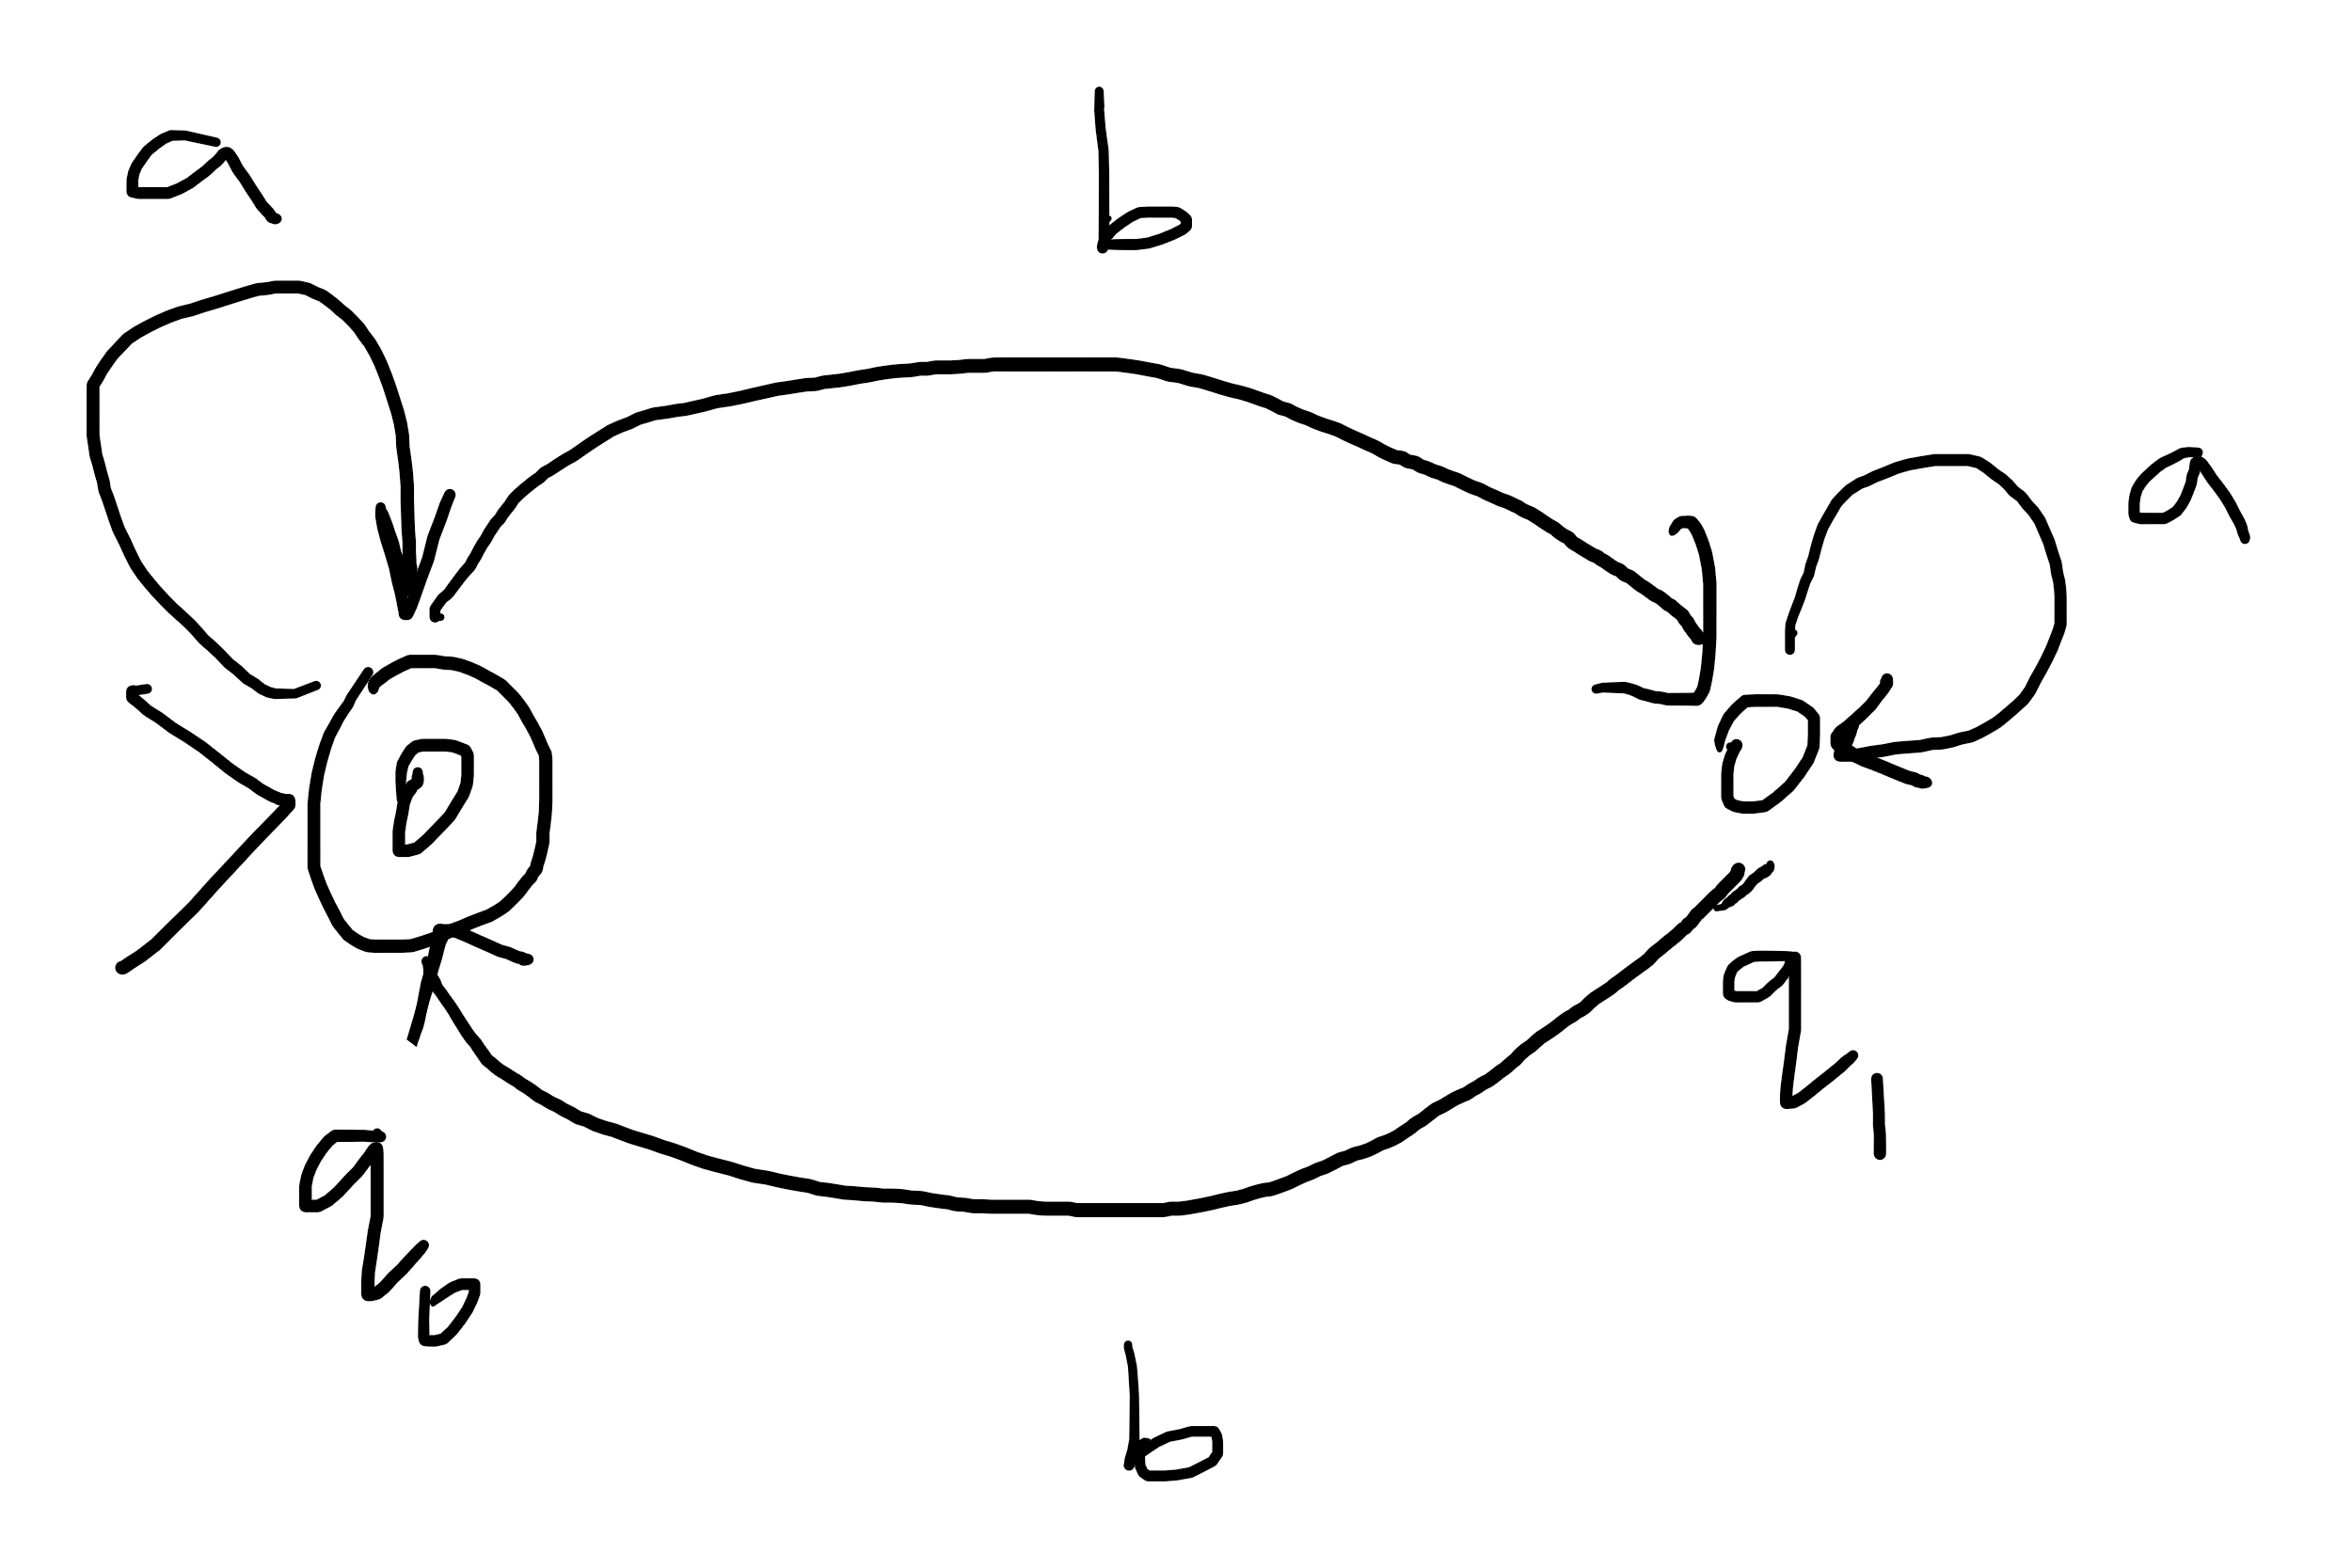
\includegraphics[width=0.4\linewidth]{std1.png}
  \label{fig:test1}
\end{figure}
\begin{definition}
	A \textbf{nondeterministic finite automaton} is a also a quintuple $M = (\Sigma,K,\Delta,s,F)$, in which everything is the same as it was for deterministic automata, except that the transition function $\Delta$ is no longer required to be a function but is relaxed to being a relation. In fact, it is also allowed to take free steps without 'consuming' characters on the input tape, i.e. $\Delta \subseteq K \times (\Sigma \cup \{\epsilon\}) \times Q$. Each triple $(q,u,p)$ is called a \textbf{transition} of $M$. Again as before, a \textbf{configuration} of $M$ is a pair $(q,\sigma) \in K \times \Sigma^*$. Again almost as before, $c_1 = (q,w),c_2 = (q',w')$ are configurations, then we say that configuration $c_1$ \textbf{yields in one step} configuration $c_2$ if there is a $u \in \Sigma \cup \{\epsilon\}$ such that $w=uw'$ and $(q,u,q') \in \Delta$. As before we also define the \textbf{yields} relation as the reflexive transitive closure of the yields in one step relation. We say that a string $w \in \Sigma^*$ is \textbf{accepted} by $M$ if there is a state $q \in F$ such that $(s,w)$ yields $(q,\epsilon)$. Finally, $L(M)$, denoting \textbf{the language accepted by} $M$, is the collection of all strings accepted by $M$.
\end{definition}
Note that any deterministic finite automaton is also a nondeterministic finite automaton, and in this special case the definitions of configurations, acceptance, and yielding are coincide. On the other hand, a nondeterministic finite automaton can be seen as a deterministic finite automaton if and only if the transition relation is a function from $K \times \Sigma$ to $K$, i.e. it contains no triplets of the form $(q,\epsilon,p)$, and for each $q \in K, a \in \Sigma$ there is exactly one $p \in K$ such that $(q,a,p) \in \Delta$. It can also easily be checked via a state diagram: the state diagram of a finite automata is deterministic iff
\begin{itemize}
	\item[1] There are no 'free' movements (i.e. no $e$ edges, which are intuitively state transition which can be made without consuming the current character of the string being evaluated)
	\item[2] For each node, there is exactly one transition leaving the node for each character in the machine's alphabet. Bear in mind that a nondeterministic machine could have more than one, or even $0$.
\end{itemize} 
Clearly the class of languages accepted by deterministic finite automata is a subset of the class defined via nondeterministic finite automata. We say that two finite automata $M_1,M_2$ (nondeterministic or deterministic) are \textbf{equivalent} if $L(M_1) = L(M_2)$. We now have that any deterministic finite automaton is equivalent to a nonderministic finite automaton, namely itself. The surprise is the converse:
\begin{theorem}
	For any nondeterministic finite automaton $M$, there exists an equivalent deterministic finite automaton $M'$.
\end{theorem}
\begin{proof}
	Let $M=(K,\Sigma,\Delta,F)$ be a nondeterministic finite automaton. We shall construct the deterministic finite automaton $M=(K',\Sigma',\delta,F')$. The new set of states $K'$ shall be the power set of the old one, i.e. $K'=2^K$. Furthermore $F'$ will be the subset of collections of states which include at least one state in the original $F$. Next, for any state $q \in K$, we let $E(K)$ be the set of all states of $M$ that are reachable from $q$ without reading any inputs, i.e.
	\[ E(q) = \{p \in K: (q,\epsilon) \overset{M^*}{\to} (p,\epsilon)\} \]
Alternatively, $E(q)$ is the closure of $\{q\}$ under the relation $\{(p,r): \textrm{ there exists a transition } (p,e,r) \in \Delta \}$. We use this to define the new starting state: $s' = E(s)$. We also use this to define the transition function: For $Q \in K'$ (capital because equivalently $Q \subseteq K$), let 
\[ \delta(Q,a) = \bigcup\{ E(p): p \in K \wedge (q,a,p)\in \Delta \textrm{ for some }q\in Q \} \] 
I.e. $\delta(Q,a)$ is the collection of all states of $M$ which $M$ can transition to after reading an $a$. This defines the clearly deterministic machine $M'$.
\par We claim that for any string $w \in \Sigma^*$ and any states $p,q \in K$, that for some $P$ containing $p$,  
\[ (q,w) \overset{M^*}{\to} (p,\epsilon) \iff (E(q),w) \overset{M'^*}{\to} (P,\epsilon) \]
From this claim, it follows that $M'$ and $M$ are equivalent. Indeed, for any $w \in \Sigma^*$, $w \in L(M)$ iff $(s,w)$ yields $(f,\epsilon)$ for some $f \in F$. But if the claim is true, this is true iff $(E(s)=s',w)$ yields $(F,\epsilon)$ for some $F$ containing $f$, but then $F \in F'$. Thus $M$ accepts $w$ iff $M'$ accepts $w$, and we have equivalency. We prove the claim by induction on the length of $w$. If $|w| = 0$, then $w = \epsilon$. Suppose that $(q,\epsilon)$ yields (via $M$) $(p,\epsilon)$. Note then that this is equivalent to saying that $p \in E(q)$. Note next that $(E(q),\epsilon)$ yields (by $M'$) $(P,\epsilon)$ for some $P$ containing $p$ iff $E(q) = P$, and of course $p \in E(q)$. Thus the equivalence holds for $w = \epsilon$.
\par Now, suppose that for strings $v$ of length $k$, we have $(q,w) \overset{M^*}{\to} (p,\epsilon) \iff (E(q),w) \overset{M'^*}{\to} (P,\epsilon)$. Let $w = va$, where $a \in \Sigma$. I.e. $w$ is an arbitrary string of length $k+1$. Suppose $(q,w) \overset{M^*}{\to} (p,\epsilon)$. Then there are states $r_1$ and $r_2$ such that
\[ (q,w) \overset{M^*}{\to} (r_1,a) \overset{M}{\to} (r_2,\epsilon) \overset{M}{\to} (p,\epsilon) \]
Now $(q,va) \overset{M^*}{\to} (r_1,a)$ amounts to $(q,v) \overset{M^*}{\to} (r_1,e)$, and since $|v|=k$, by the inductive hypothesis we have that $(E(q),v) \overset{M'^*}{\to} (R_1,\epsilon)$ for some $R_1$ containing $r_1$. Since $(r_1,a) \overset{M}{\to} (r_2, \epsilon)$, there exists a triple $(r_1,a,r_2) \in \Delta$, and thus by definition of $\delta$ we have that $E(r_2) \subseteq \delta(R_1,a)$. But since $(r_2,\epsilon) \overset{M^*}{\to} (p,\epsilon)$, it follows that $p \in E(r_2)$, and thus $p \in \delta(R_1,a)$. Thus, $(R_1,a) \overset{M'}{\to} (P,\epsilon)$, for some $P$ containing $p$, and thus $(E(q),va)\overset{M'^*}{\to} (R_1,a) \overset{M'}{\to} (P,\epsilon)$.
\end{proof}
Note that since this proof is constructive, it follows that one can always design deterministic finite automata by first designing a nondeterministic one and then following the outline detailed above to create from it a deterministic one. Also because of this lack of distinction, we can drop the distinction between deterministic and nondeterministic automata altogether now and simply refer to finite automata. Not only that, we can go back and forth between the deterministic and nondeterministic models, using whatever is convenient (usually the nondeterministic).
\begin{lemma}
	The class of languages accepted by finite automata is closed under union, concatenation, Kleene star, complementation, and intersection.
\end{lemma}
\begin{proof}
	For union, let $M_1 = (\Sigma,K_1,\Delta_1,s_1,F_1),M_2 = (\Sigma,K_2,\Delta_2,s_2,F_2)$. (It only makes sense to think of these machines as having the same alphabet considering we are really thinking about their union, which will involve both. Since nondeterministic machines are not required to have an edge for every symbol, one can always think of them as being over a larger alphabet then that actually are.) Consider the machine 
	\[ M=(\Sigma,K_1 \cup K_2 \cup \{e\},\Delta_1 \cup \Delta_2 \cup \{(s,e,s_1),(s,e,s_2)\},s,F_1 \cup F_2) \]
What is the behavior of this machine? For a given input, it simply guesses whether to transition to the first or second computation, and runs that. Clearly $x \in L(M) \iff x \in L(M_1) \cup L(M_2)$, and so $L(M) = L(M_1)\cup L(M_2)$. \par 
	Next, concatenation. Let $M_1$ and $M_2$ be as above. Let 
	\[ M = (\Sigma,K_1 \cup K_2,\Delta,s_1,F_2) \]
	Where $\Delta$ contains all of the transitions of both $\Delta_1$ and $Delta_2$, but in addition has all transitions $(f,e,s_2)$ such that $f \in F_1$. Thus the behavior of this machine is to simulate the behavior of $M_1$ for a while, and then nondeterministically jumping from the final state of that computation to the initial state of the second computation. $x \in L(M_1)L(M_2)$ iff $x = yz$ where $y \in L(M_1),z \in L(M_2)$ iff there is a state $q_1 \in F_1$ such that $(s_1,y) \overset{M^*}{\to} (q_1,e)$ (iff $(s_1,yz) \overset{M^*}{\to} (q_1,z)$) and there is a state $q_2 \in F_2$ such that $(s_2,z) \overset{M^*}{\to} (q_2,e)$, and the nondeterministic jump from every final state of $M_1$ to $M_2$ ensures that the above is true iff $x \in L(M)$. \par    
	The construction for Kleene star is very similar to what we did above for concatenation so we won't list out all of the details, and instead only describe it. To construct a machine $M$ such that $L(M) = L(M_1)^*$, we take $M_1$ and add to it a new starting state $s$, as well as adding transitions of the form $(f,e,s)$ to $\Delta_1$ for any $f \in F_1$. We also make sure that this new starting state is also a final state, so that $e \in L(M)$. We also add the transition $(s,e,s_1)$ so that the machine can transition from the new actual starting state to the old starting state for free. It's clear that what we've constructed is a machine which will simulate $M_1$ repeatedly, some guessed number of times until the string is empty, and accept iff the string is in $L(M_1)^*$. \par 
	Closure over intersections will follow from deMorgan's laws and closure under complementation, which it remains to show. Towards this, it will be easier to begin with a deterministic finite machine $M = (\Sigma,K,\delta,s,F)$. Consider the machine $\bar{M} = (\Sigma,K,\delta,s,K-F)$, i.e. the machine in which all of the nonfinal states are now final states and vice versa. For any deterministic machine it must be the case that $(s,x) \overset{M^*}{\to} (q,e)$ for some $q$, but now this $q$ will be in the final states of $\bar{M}$ iff it is not in the final state for $M$, i.e. iff it is in $L(M)^c$, and so $L(\bar{M}) = L(M)^c$. 
\end{proof}
Recall our observation earlier that the regular languages were the closure of the set $\{\{\sigma \}: \sigma \in \Sigma\} \cup \{\varnothing \}$ under the union, concatenation, and Kleene star operations - that is to say, the smallest set containing this initial set and closed under all of these operations. Clearly the very dumb state diagrams drawn below show nondeterministic Turing machines which decide the singleton languages as well as the empty language.
\begin{figure}[H]
	\centering
  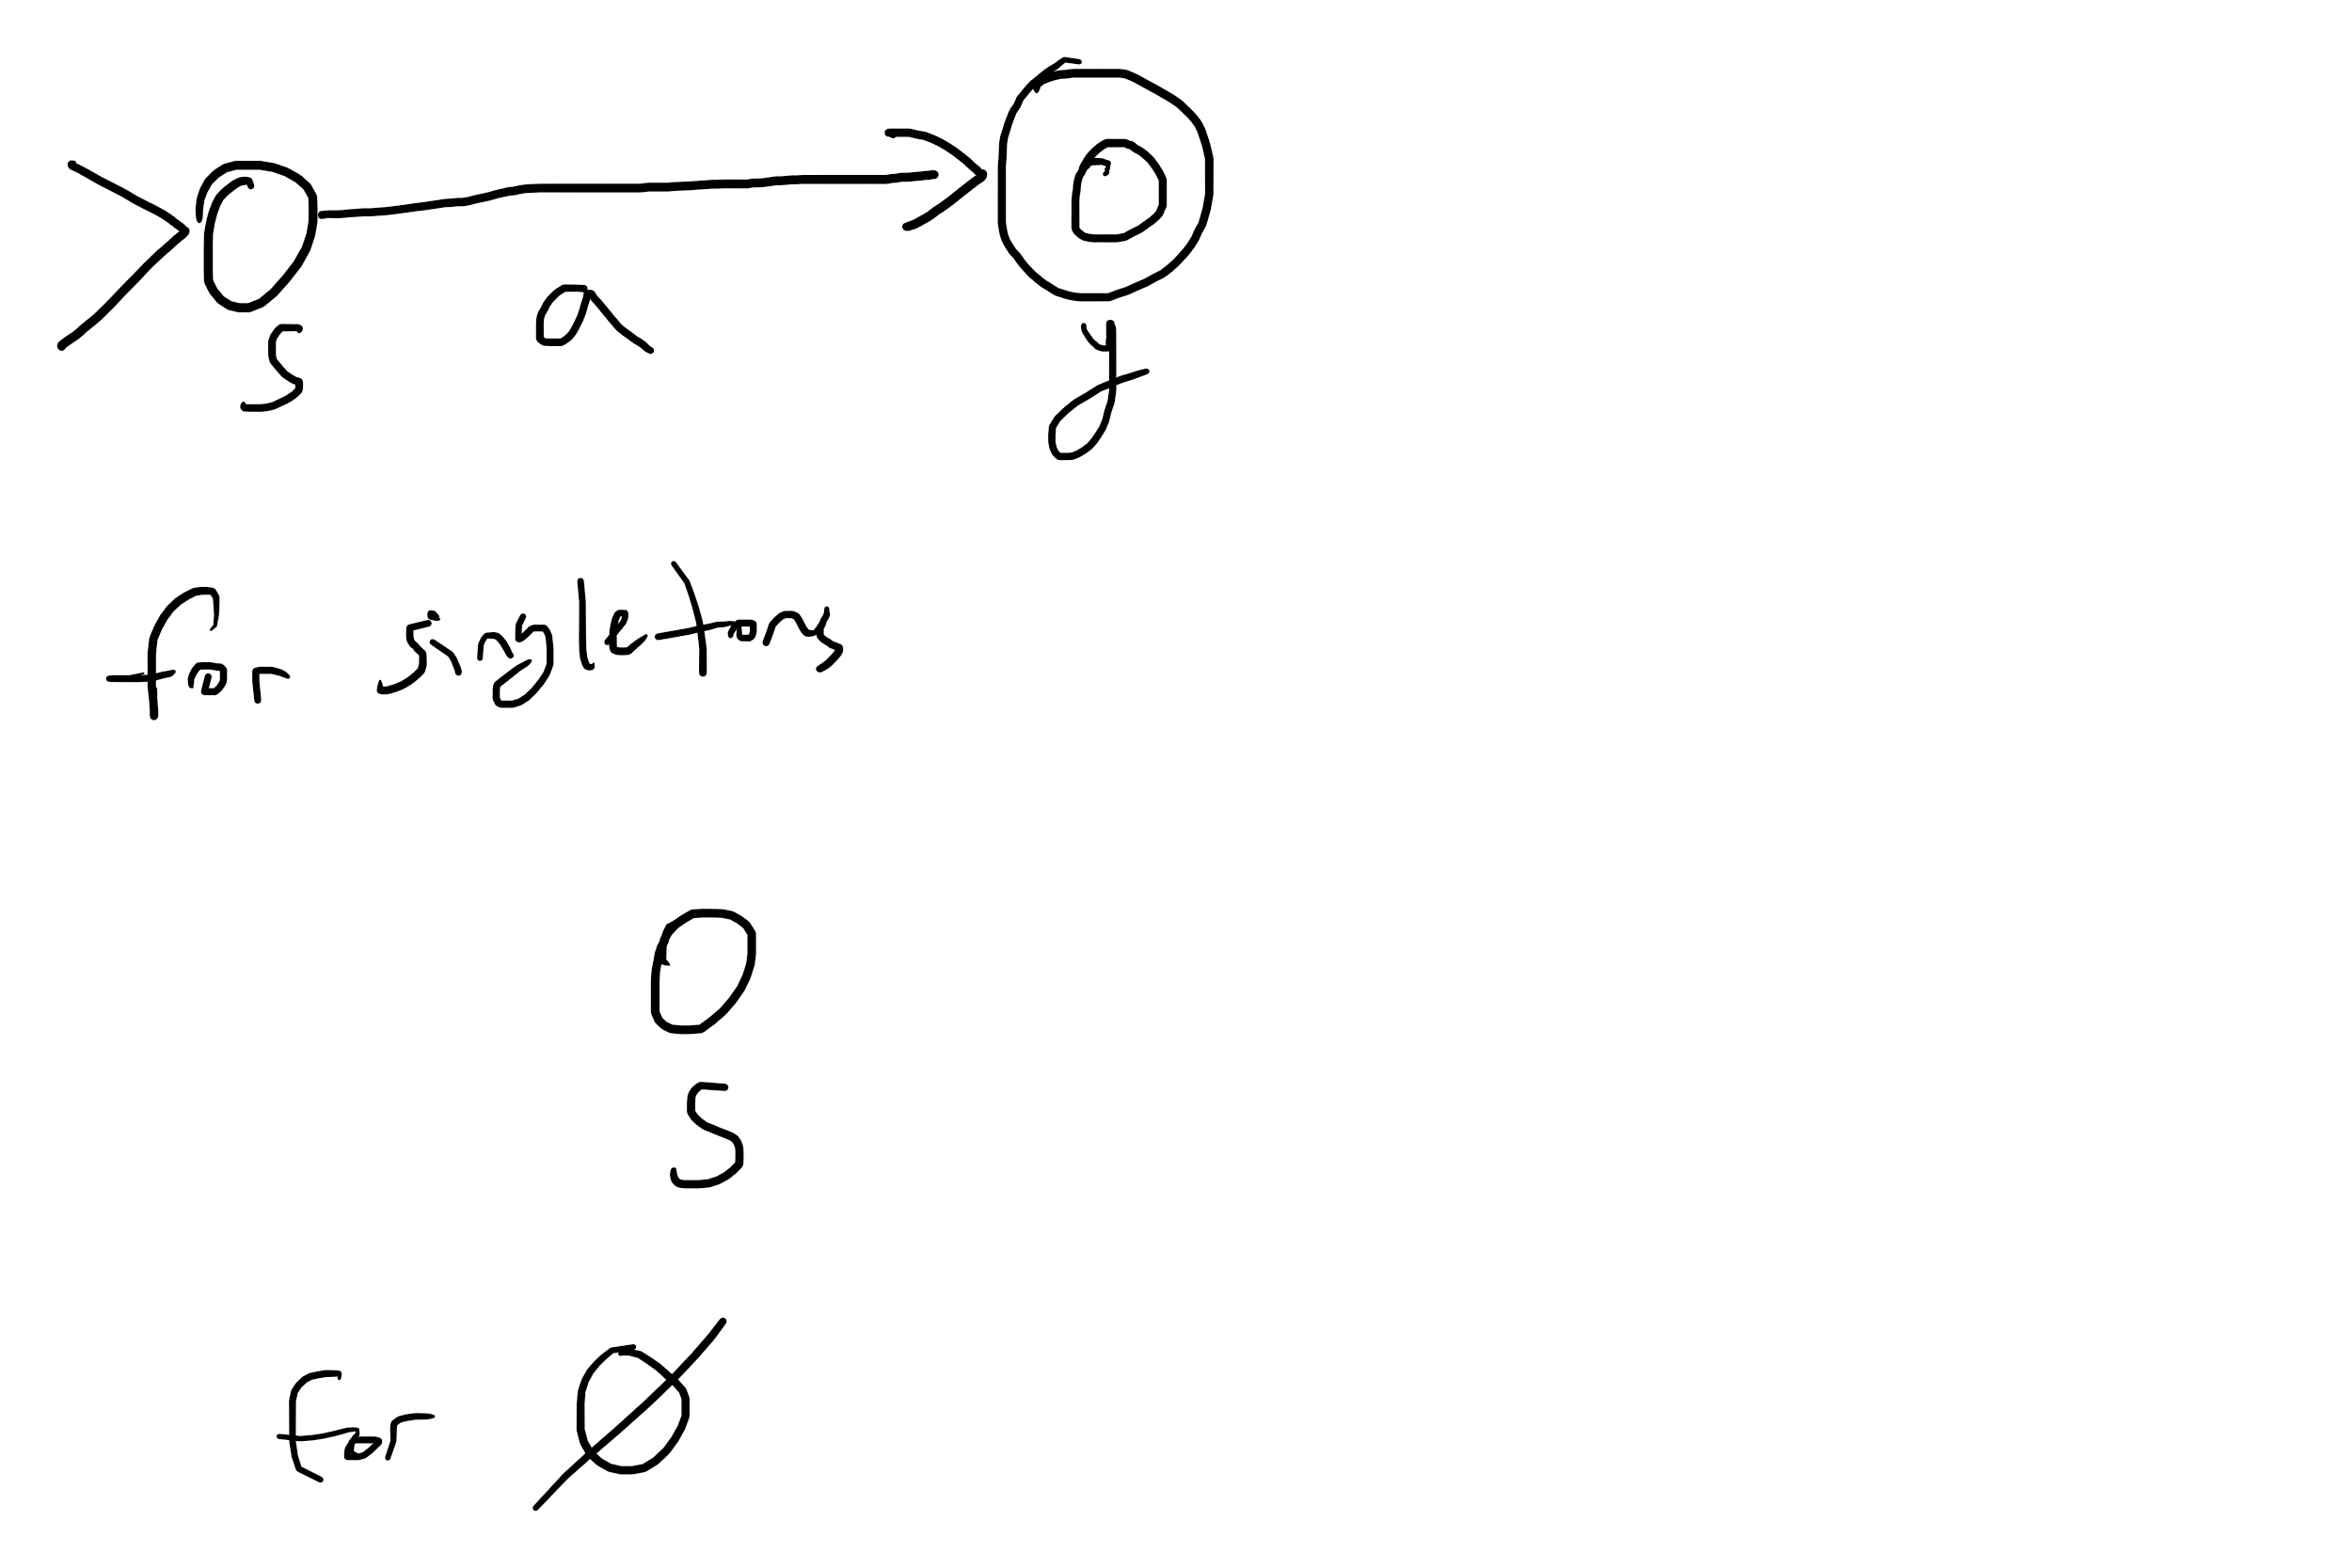
\includegraphics[width=0.4\linewidth]{dumb.png}
  \label{fig:test1}
\end{figure}
Thus as a corollary to this lemma we must conclude that the set of languages acceptable by finite automata contains the set of regular languages. 
\begin{lemma}
	Let $M$ be an arbitrary finite automata. Then $L(M)$ is regular
\end{lemma}
\begin{proof}
	Let $M = (\Sigma,K,\Delta,s,F)$ (it could be deterministic or not, doesn't matter). Let $K = \{q_1,...,q_n\}$ with $s = q_1$. For $i,j = 1,...,n$, and $k=0,1,...,n$, define $R(i,j,k)$ to be the collection of strings $x$ such that some block of transitions within the computation of $x$ will take the state $q_i$ to the state $q_j$ without ever entering into any of the states $q_{k+1},q_{k+2},...,q_n$ (the indices of $q_i$ and $q_j$ themselves are allowed to be anything though). More formally, $R(i,j,k)$ is the set of all $x = x_1x_2\ldots x_m$ such that for some $\alpha,\beta \in \{1,2,...,m-1\}$ with $\beta \geq \alpha$, $(q_i,x_{\alpha}x_{\alpha+1}\ldots x_m) \overset{M^{\beta-\alpha}}{\to} (q_j,x_{\beta}x_{\beta+1}\ldots x_m)$, and such that it is not the case that $(q_i,x_{\alpha}x_{\alpha+1}\ldots x_m)\overset{M^{\gamma}}{\to} (q_t,x_{\alpha-\gamma}x_{\alpha-\gamma+1}\ldots x_m)$ for any $\gamma = 1,...,\beta-\alpha, t>k$. The formalization doesn't matter at all, it's just here to convince the reader that this definition is rigorous. \par 
	First note that when $k=n$, $R(i,j,k) = \{w \in \Sigma^*: (q_i,w) \overset{M^*}{\to} (q_j,e)\}$, and so $L(M) = \bigcup_{q_j \in F} R(1,j,n)$. This is a finite union, and so if we can show that $R(i,j,k)$ is regular for every $i,j,k$, then by closure of regular languages under finite unions we are done. We go by induction on $k$. \par 
	For $k=0$, $R(i,j,0) = \{a \in \Sigma \cup \{e\}: (q_i,a,q_j) \in \Delta \}$, if $i\neq j$, and if $i=j$ it's the same set unioned with $\{e\}$. Either way this set is finite, and thus regular since singletons are regular and regular languages are closed under finite unions. Now suppose that $R(ij,k-1)$ have been observed as regular for all $i,j$. Observe the following expression for $R(i,j,k)$, which we will justify after:
	\[R(i,j,k) = R(i,j,k-1) \cup R(i,k,k-1)R(k,k,k-1)^*R(k,j,k-1) \]
To get from $q_i$ to $q_j$, we can get there by transitioning without using any states greater than $k-1$, \textit{or} by first going from state $q_i$ to $q_k$, \textit{then} going from $q_k$ to $q_k$ again one or more times, and \textit{then} going from $q_k$ to $q_j$. (Observe that the middle path could entail states below $k$, so $q_k$ can be used anywhere in the path as many times as necessary). By the inductive hypothesis and since regular languages are closed under unions, concatenation and Kleene star, it follows that $R(i,j,k)$ is regular, completing the induction and subsequently the proof. 
\end{proof}
We thus have the following major result:
\begin{theorem}
	A language is regular if and only if it is accepted by a finite state machine. That is to say, the class of languages accepted by finite state machines is precisely the class of regular languages. 
\end{theorem}
[Add general method for producing a regular language from finite state machine] \\
The next theorem will help us understand the limits of regular languages in terms of expressiveness, and simultaneously as a result of the above theorem will help understand the limits of the computational power of finite automata.
\begin{theorem}
	Let $L$ be a regular language. Then there is an integer $n \geq 1$ such that any string $w \in L$ with $|w| \geq n$ can be rewritten $w=xyz$ such that $y \neq e$, $|xy| \leq n$, and $xy^iz \in L$ for each $i \geq 0$.
\end{theorem}
\begin{proof}
	Since $L$ is regular, $L$ is accepted by a deterministic finite automata $M$. Suppose that $n$ is the number of states of $M$ and let $w$ be a string of length $n$ or greater which is accepted by $L$. Consider now the first $n$ steps of the computation of $M$ on $w$:
	\[ (w_1w_2\ldots w_n,q_0) \overset{M}{\to} (w_2\ldots w_n,q_1) \overset{M}{\to} \ldots \overset{M}{\to} (e,q_n) \] 
	Here $q_0$ is the initial state and $w_1\ldots w_n$ is the initial length $n$ segment of $w$. By the pigeonhole principle there has to exist an $i,j \leq n$ such that $q_i = q_j$. Consider the implications of this on the substring $y = w_iw_{i+1} \ldots w_j$. This substring drives $M$ to the same place where it started, and can be inserted repeatedly without changing the resulting computation of $M$. It could be removed from $w$ or repeated any finite number of times, and nothing would change. That is to say, if we let $x = w_1w_2\ldots w_{i-1}$ and $z = w_{j+1}\ldots w_n$, then $w = xyz$, and $xy^iz$ is accepted by $L$ for any $i \in \mathbb{N}$. 
\end{proof}
As an example of the using this fact, consider the language $L = \{a^ib^i: i \geq 0\}$. If this language were regular, then there would exist an $n$ such that the above theorem holds. But then if we let $w = a^nb^n$, this is clearly in $L$, but then by the theorem can be written $w = xyz$ where $y \neq e$ and $|xy| \leq n$. But then $xy = a^i$ for some $i \leq n$, and by the theorem it would need to be the case that $a^{n-i}b^n \in L$, which it isn't. Thus $L$ is not regular. \par 
Since regular Turing machines can obviously decide this language, it follows that finite state machines are a strictly weaker model of computation than Turing machines. This fact is so predictable that we don't even bother to state it as a corollary. \par 
Another example. Let $L = \{a^n: \textrm{ n is prime}\}$. Suppose this were regular, let $n$ be as above, and $w \in L$, with $x,y,z$ picked appropriately so $w = xyz$ with all of the properties we specified. Then of course $x = a^p$, $y = a^q$, and $z=a^r$, where $p,r \geq 0$, $q > 0$. Then $xy^iz \in L$ for each $i$, but this would imply that $p+iq+r$ is prime for every $i$. Letting $i=p+2q+r+2$, we get that $p+(p+2q+r+2)q+r$ is prime. But this simplifies to $(q+1)(p+2q+r)$, the product of two nontrivial numbers, and so is not prime, a contradiction. Thus $L$ cannot be regular. \par 
One final example building on the previous: Consider $L = \{w \in \{a,b\}^*: \textrm{ w has an equal number of $a$'s and $b$'s}\}$. Suppose this were regular. Then $L \cap a^*b^*$ would also be regular since the regular languages are closed under intersection. But this language is precisely $\{a^nb^n: n \geq 0\}$, which we already demonstrated was not regular. 
\section{Context-Free Languages and Pushdown Automata}
\begin{definition}
	A \textbf{context free grammar} is a quadruple $G = (V,\Sigma,R,S)$, where $V$ is a finite alphabet, $\Sigma \subset V$ is called a set of \textbf{terminals}, $R \subseteq (V-\Sigma) \times V^*$ is a relation called the set of \textbf{rules}, and $S \in V-\Sigma$ is called the \textbf{start symbol}. The members of $V-\Sigma$ are called \textbf{nonterminals}. For any nonterminal $A \in V - \Sigma$ and $u \in V^*$, we write $A \to_G u$ whenever $(A,u) \in R$. For any strings $u,v \in V^*$, we write $u \implies_G v$ if there exist strings $x,y \in V^*$ and a nonterminal $A \in V-\Sigma$ such that $u = xAy, v = xv'y$ and $A \to_G v'$. The relation $\implies^*_G$ is defined as the reflexive, transitive closure of $\sigma_G$. Finally, \textbf{the language generated by G} is defined 
	\[ L(G) = \{w \in \Sigma^*: S \implies^*_G w\} \]
If $x \in L(G)$, we say that $G$ \textbf{generates} the string $x$. Finally, a language $L$ is said to be \textbf{context-free} if $L = L(G)$ for some context free grammar $G$. 
\end{definition}
When the grammar is obvious we will write $\to$ and $\implies$ without the $G$ subscript. We call any sequence of the form 
\[ w_0 \implies w_1 \implies \ldots \implies w_n \]
A \textbf{derivation} in $G$ of $w_n$ from $w_0$. 
As an example, consider $G = (V,\Sigma,R,S)$, where $V = \{S,a,b\}$, $\Sigma = \{a,b\}$, $R = \{(S,aSb),(S,e)\}$. Recall these relation elements correspond to the rules $S \to aSb$ and $S \to e$, and we will usually write these as the elements instead. What is $L(G)$? Suppose $x \in L(G)$. Then $S \implies^* x$. First of all, $e \in L(G)$, since that is a one rule derivation. The only other option is for $S \implies aSb$ to be the first rule used, in which case there is again, only ever one option: either add another $a$ and $b$ on the left and right sides, or terminate. Thus it is clear that $L(G) = \{a^nb^n: n \in \omega\}$. Thus we have the following:
\begin{corollary}
	Not all context-free languages are regular.
\end{corollary}
Are all regular languages context-free? There are a variety of ways in which we would like to demonstrate this. First, let us look at regular languages as a special restricted type of context-free grammar. Call a context-free grammar \textbf{regular} (or \textbf{right-linear}) if, instead of $R \subseteq (V - \Sigma)\times V^*$, we instead require that $R \subseteq (V-\Sigma) \times \Sigma^*(V-\Sigma \cup \{e\})$. That is, whereas with ordinary context-free grammars, nonterminals can derive to arbitrary strings over $V$, with regular grammars the nonterminals are restricted to deriving to the specific form of a string of terminals followed by at most a single nonterminal. 
\begin{definition}
	A \textbf{pushdown automaton} is a sextuple $M = (Q,\Sigma,\Gamma,\Delta,s,F)$, where $Q$ is a finite set of \textbf{states}, $\Sigma$ and $\Gamma$ are finite alphabet, with those of $\Sigma$ being called the \textbf{input symbols} and those of $\Gamma$ being called the \textbf{stack symbols}, $s \in Q$ is the \textbf{initial state}, $F \subseteq Q$ is the set of \textbf{final states}, and $\Delta \subseteq (Q \times (\Sigma \cup \{e\}) \times \Gamma^*) \times (Q \times \Gamma^*)$ is called the \textbf{transition relation}.
\end{definition}
Intuitively, if $((p,a,\beta),(q,\gamma)) \in \Delta$, then $M$, whenever it is in state $p$ with $\beta$ at the top of the stack, may read $a$ from the input tape (if $a = e$ then the input is not consulted), replace $\beta$ by $\gamma$ at the top of the stack, and enter state $q$. Such a pair $((p,a,\beta),(q,\gamma))$ is called a \textbf{transition} of $M$; since several transitions of $M$ may be simultaneously applicable at any point, the machines we are describing are nondeterministic in operation. (Later we will restrict this definition to define the deterministic pushdown automata, which will prove, unlike in the case of finite state automata, to be a strictly weaker class of objects.) \par 
To \textbf{push} a symbol is to add it to the top of the stack. To \textbf{pop} a symbol is to remove it from the top of a stack. For example, the transition $((p,u,e),(q,a))$ pushes $a$, while $((p,u,a),(q,e))$ pops $a$. \par 
As in the case with finite automata, during the computation the portion of the input already read does not affect the subsequent operation of the machine. Accordingly, a \textbf{configuration} of a pushdown automaton is defined to be a member of $Q \times \Sigma^* \times \Gamma^*$, where the first entry is the current state of the machine, the second is the portion of the input string yet to be read, and the third is the current contents of the pushdown store, read top-down. For example. if the configuration were $(q,w,abc)$, then $a$ would be at the top of the stack and $c$ on the bottom. If $(p,x,\alpha)$ and $(q,y,\zeta)$ are configurations of $M$, we say that $(p,x,\alpha)$ \textbf{yields in one step} $(q,y,\zeta)$, and denote this $(p,x,\alpha) \to_M (q,y,\zeta)$, if there is a transition $((p,a,\beta),(q,\gamma)) \in \Delta$ such that $x = ay$ and $\alpha = \beta \eta$ and $\zeta = \gamma \eta$ for some $\eta \in \Gamma^*$. The symbols are a bit confusing here - $\alpha$ and $\beta$ here are the complete contents of the stack from step one to step two. $\beta$ is an initial segment of $\alpha$ (with the rest of the stack labeled $\eta$, which is to be popped, and $\gamma$ is a new initial segment, to be pushed, resulting in the stack contents $\gamma \eta$, which is equal to $\zeta$, the final contents of the stack at the end of the step. \par 
Of course, from here we can define $\to^*_M$ as the reflexive transitive closure of $\to_M$. We can similarly define that $M$ \textbf{accepts} a string $w \in \Sigma^*$ if $(s,w,e) \to^*_M (p,e,e)$ for some state $p \in F$. To put it another way, $M$ accepts $w$ if there is a sequence of configurations $c_1,c_2,...,c_n$ with $n > 0$ such that $c_0 \to_M c_1 \to_M \ldots \to_M c_n$ where $c_0 = (s,w,e)$ and $c_n = (p,e,e)$ for some $p \in F$. The sequence itself $c_0,c_1,...,c_n$ is called the \textbf{computation} by $M$, and $n$ is the number of \textbf{steps} of the computation. Finally, the \textbf{language accepted by $M$}, denoted $L(M)$, is the set of all strings accepted by $M$. \par 
Note that any finite automaton can be trivially viewed as a pushdown automaton which never operates on it's stack. To make this precise, let $M = (Q,\Sigma,\Delta,s,F)$ be a nondeterministic finite automaton, and let $M'$ be the pushdown automaton $(Q,\Sigma,\varnothing,\Delta',s,F)$, where $\Delta' = \{((p,u,e),(q,e)): (p,u,q) \in \Delta\}$. That is to say, $M'$ is a pushdown automaton which always pushes and pops the empty string on its stack, and otherwise simulates the transitions of $M$. Then immediately from the definitions it should obviously follow that $L(M') = L(M)$. 
\section{Grammars and Turing Machines}
I'm assuming that the reader has already seen my regular computability notes and knows the definition of recursive enumerability and Turing machines. With context-free grammars, the pivotal element was the set of rules, defined to be a relation $R \subseteq V-\Sigma \times V^*$. The 'context-free' comes from the fact that rules specifically map the non-terminals to new strings over the vocabulary - \textit{irrespective} of any surrounding symbols. To introduce context-\textit{dependency} then, would be to take the \textit{entire} string (provided there is at least one nonterminal symbol somewhere), and replace it all at once. That is to say, for grammars in general, $R \subseteq V^*(V-\Sigma)V^* \times V^*$. We now state the entire definition formally:
\begin{definition}
	A \textbf{grammar} (or \textbf{unrestricted grammar}, or a \textbf{rewriting system} is a quadruple $G = (V,\Sigma,R,S)$, where $V$ is an alphabet, $\Sigma \subseteq V$ is the set of \textbf{terminal} symbols, $V - \Sigma$ is the set of \textbf{nonterminal symbols}, $S \in V-\Sigma$ is the \textbf{start symbol}, and $R \subseteq V^*(V-\Sigma)V^* \times V^*$ is a finite set of \textbf{rules}. (Note it must be explicitly restricted to being finite - in the case of context free grammars this was not a concern.) \par 
	We write $u \to v$ to denote the $(u,v) \in R$. We write $u \implies v$ iff, for some $w_1,w_2 \in V^*$, and some rule $u' \to v' \in R$, we have that $u = w_1u'w_2$ and $v = w_1v'w_2$. (So we can apply a rule to any chunk of any string.) As usual, $\implies^*$ is the reflexive, transitive closure of $\implies$. A string $w \in \Sigma^*$ is \textbf{generated} by $G$ iff $S \implies^* w$ - an explicit sequence of single step $\implies$ which accomplish this is called a \textbf{derivation} of $w$. Finally, the \textbf{language generated by $G$}, denoted $L(G)$, is the set of all strings generated by $G$. 
\end{definition}
\end{document}
